% ---------------------------------------------------------------------------
% ---------------------------------------------------------------------------
% Modelo LaTex para preparação do documento final de Monografia TCC
% O modelo está em conformidade com ABNT NBR
% Faculdade do Piaui
% ---------------------------------------------------------------------------
% ---------------------------------------------------------------------------

\documentclass[
	% -- opções da classe memoir --
	12pt,					% tamanho da fonte
	openright,				% capítulos começam em pág ímpar (insere página vazia caso preciso)
	twoside,					% para impressão em verso e anverso. Oposto a oneside
	a4paper,					% tamanho do papel. 
	% -- opções da classe abntex2 --
	%chapter=TITLE,			% títulos de capítulos convertidos em letras maiúsculas
	%section=TITLE,			% títulos de seções convertidos em letras maiúsculas
	%subsection=TITLE,		% títulos de subseções convertidos em letras maiúsculas
	%subsubsection=TITLE,	% títulos de subsubseções convertidos em letras maiúsculas
	% -- opções do pacote babel --
	english,					% idioma adicional para hifenização
	%french,					% idioma adicional para hifenização
	%spanish,				% idioma adicional para hifenização
	brazil					% o último idioma é o principal do documento
	]{abntex2}

% ---------------------
% Pacotes OBRIGATÓRIOS
% ---------------------
\usepackage{lmodern}				% Usa a fonte Latin Modern			
\usepackage[T1]{fontenc}			% Selecao de codigos de fonte.
\usepackage[utf8]{inputenc}		% Codificacao do documento (conversão automática dos acentos)
\usepackage{lastpage}			% Usado pela Ficha catalográfica
\usepackage{indentfirst}			% Indenta o primeiro parágrafo de cada seção.
\usepackage{color}				% Controle das cores
\usepackage{graphicx,graphicx}	% Inclusão de gráficos
\usepackage{epsfig,subfig}		% Inclusão de figuras
\usepackage{microtype} 			% Melhorias de justificação
\graphicspath{{figs/}}
\usepackage[table,xcdraw]{xcolor}
% ---------------------
		
% ---------------------
% Pacotes ADICIONAIS
% ---------------------
\usepackage{pdfpages}


\usepackage{lipsum}						% Geração de dummy text
\usepackage{amsmath,amssymb,mathrsfs}	% Comandos matemáticos avançados 
\usepackage{setspace}  					% Para permitir espaçamento simples, 1 1/2 e duplo
\usepackage{verbatim}					% Para poder usar o ambiente "comment"
\usepackage{tabularx} 					% Para poder ter tabelas com colunas de largura auto-ajustável
\usepackage{afterpage} 					% Para executar um comando depois do fim da página corrente
\usepackage{url} 						% Para formatar URLs (endereços da Web)

%\usepackage[style=long,nonumberlist,toc,xindy,nomain]{glossaries}
				% para fazer glossario	
\usepackage{glossaries}	
\loadglsentries{extras/glossary}
\makeglossaries

%% para referenciar abreviaturas
\makeatletter
\def\namedlabel#1#2{\begingroup
	#2%
	\def\@currentlabel{#2}%
	\phantomsection\label{#1}\endgroup
}
% ---------------------

% ---------------------
% Pacotes de CITAÇÕES
% ---------------------
\usepackage[brazilian,hyperpageref]{backref}	% Paginas com as citações na bibl
\usepackage[alf]{abntex2cite}				% Citações padrão ABNT (alfa)
%\usepackage[num]{abntex2cite}				% Citações padrão ABNT (numericas)
% ---------------------

\usepackage{ulem}

\definecolor{mypurple}{rgb}{0.8,0.5,1}
\newcommand{\fulano}[1]{\textcolor{mypurple}{#1}}
\definecolor{mygreen}{RGB}{28,172,0} % color values Red, Green, Blue
\definecolor{mylilas}{RGB}{170,55,241}
\newcommand{\source}[1]{\caption*{Fonte: {#1}} }

% Configurações de CITAÇÕES para abntex2
% --- 
% CONFIGURAÇÕES DE PACOTES
% --- 

% ---
% Configurações do pacote backref
% Usado sem a opção hyperpageref de backref
\renewcommand{\backrefpagesname}{Citado na(s) página(s):~}
% Texto padrão antes do número das páginas
\renewcommand{\backref}{}
% Define os textos da citação
\renewcommand*{\backrefalt}[4]{
	\ifcase #1 %
		Nenhuma citação no texto.%
	\or
		Citado na página #2.%
	\else
		Citado #1 vezes nas páginas #2.%
	\fi}%
% ---

% Inclusão de dados para CAPA e FOLHA DE ROSTO (título, autor, orientador, etc.)
% ---
% Informações de dados para CAPA e FOLHA DE ROSTO
% ---
\titulo{Algoritmo para correção de tom por meio da análise em frequência}
\autor{
	Cleber Couto Filho\\
	Ícaro Nascimento Queiroz\\	
}
\local{Salvador-BA}
\data{\today}

\instituicao{%
  Centro Universitário SENAI CIMATEC}
\tipotrabalho{Avaliação}
% O preambulo deve conter o tipo do trabalho, o objetivo,
% o nome da instituição e a área de concentração
\preambulo{Relatório apresentado como requisito parcial para obtenção de aprovação na disciplina Processamento Digital de Sinais, no centro universitário SENAI CIMATEC.\newline \newline
	\textbf{Docente:} Leonardo Vasconsellos
	}
% ---

% Inclui Configurações de aparência do PDF Final
%  Configurações de aparência do PDF final
% NÃO ALTERAR!!!

% alterando o aspecto da cor azul
\definecolor{blue}{RGB}{41,5,195}

% informações do PDF
\makeatletter
\hypersetup{
     	%pagebackref=true,
		pdftitle={\@title}, 
		pdfauthor={\@author},
    		pdfsubject={\imprimirpreambulo},
	    pdfcreator={LaTeX with abnTeX2},
		pdfkeywords={abnt}{latex}{abntex}{abntex2}{trabalho acadêmico}, 
		colorlinks=true,       		% false: boxed links; true: colored links
    		linkcolor=blue,          	% color of internal links
    		citecolor=blue,        		% color of links to bibliography
    		filecolor=magenta,      		% color of file links
		urlcolor=blue,
		bookmarksdepth=4
} 
\makeatother
% --- 

% O tamanho da identação do parágrafo é dado por:
\setlength{\parindent}{1.3cm}

% Controle do espaçamento entre um parágrafo e outro:
\setlength{\parskip}{0.2cm}  % tente também \onelineskip

% ---------------------
% Compila o indice
% ---------------------
\makeindex
% ---------------------
\usepackage{listings}
\lstset{language=Matlab,%
	%basicstyle=\color{red},
	breaklines=true,%
	morekeywords={matlab2tikz},
	keywordstyle=\color{blue},%
	morekeywords=[2]{1}, keywordstyle=[2]{\color{black}},
	identifierstyle=\color{black},%
	stringstyle=\color{mylilas},
	commentstyle=\color{mygreen},%
	showstringspaces=false,%without this there will be a symbol in the places where there is a space
	numbers=left,%
	numberstyle={\tiny \color{black}},% size of the numbers
	numbersep=9pt, % this defines how far the numbers are from the text
	emph=[1]{for,end,break},emphstyle=[1]\color{red}, %some words to emphasise
	%emph=[2]{word1,word2}, emphstyle=[2]{style},    
}



%%%%%%%%%%%%%%%%%%%%%%%%%%%
%%  INICIO DO DOCUMENTO  %%
%%%%%%%%%%%%%%%%%%%%%%%%%%%
\begin{document}

% Retira espaço extra obsoleto entre as frases.
\frenchspacing

% ----------------------------------------------------------
% ELEMENTOS PRÉ-TEXTUAIS (Capa, Resumo, Abstract, etc.)
% ----------------------------------------------------------
\pretextual

% Capa
% ---
% Impressão da Capa
% ---
  \begin{capa}%
    \begin{figure}[h!]%
        \centering%
        
\includegraphics[scale=0.4]{figs/logo_senai.jpeg}%
      \end{figure}%
    \center
	\ABNTEXchapterfont\large{Centro Universitário SENAI CIMATEC\\Curso de Bacharelado em Engenharia Elétrica}
	%\vspace{1.5cm}

    \vfill
    \ABNTEXchapterfont\bfseries\LARGE\imprimirtitulo
    \vfill

	%\vfill
	\ABNTEXchapterfont\large\imprimirautor
	\vfill
%
    \large\imprimirlocal, \large\imprimirdata

    \vspace*{1cm}
  \end{capa}
% ---

% Folha de rosto (o * indica que haverá a ficha bibliográfica)
\imprimirfolhaderosto*

% Lista de ilustrações
\pdfbookmark[0]{\listfigurename}{lof}
\listoffigures*


% ----------------------------------------------------------
% ELEMENTOS TEXTUAIS (Capítulos)
% ----------------------------------------------------------
\textual
% Elementos textuais com numeração arábica
\pagenumbering{arabic}
% Reinicia a contagem do número de páginas
\setcounter{page}{1}

% Inclui cada capitulo da Dissertação
% ----------------------------------------------------------
% Introdução 
% Capítulo sem numeração, mas presente no Sumário
% ----------------------------------------------------------

\chapter*[Introdução]{Introdução}
\addcontentsline{toc}{chapter}{Introdução}

Este relatório descreve os procedimentos e códigos utilizados para a criação de um sistema de processamento de áudio para correção de tons musicais.

\section*{Teoria Musical}
Na música a notação utilizada, chamada diastemática, os sons são representados graficamente, de maneira que seja possível mensurar os intervalos de frequências, o que indica diferentes notas musicais. 

Para representação de sons mais longos ou curtos surge então a notação da grandeza tempo, que diferentemente da convenção comum, não possui um valor fixo, portanto, cria-se uma referência com relação à duração da notas semibreve, sendo elas a mínima, semínima, colcheia, semicolcheia, fusa, semifusa.

Outro aspecto extremamente importante da teoria musical é a frequência, grandeza qual classifica o quão graves ou agudos são os sons. Sons que apresentam maiores frequências são mais agudos que os de frequências mais baixas 

Diferentes instrumentos são capazes de gerar sons diferentes mesmo que as frequências fundamentais sejam idênticas, o que em outras palavras significa dizer que um Ré gerado por um instrumento de corda não tem o mesmo som de um Ré gerado por um instrumento de sopro ou da voz humana, Este fenômeno, que é chamado de timbre, se dá principalmente pela geometria do instrumento, que define quais serão as outras componentes senoidais adicionadas à fundamental.



\section*{Proposta}\label{sec:motivacao}

Projetar um algoritmo capaz de realizar a afinação de um som emitido pela voz humana para uma frequência selecionada através das técnicas de processamento como transformadas e mudanças de tom. Para a realização dos algoritmos foram tomadas as seguintes decisões:

\begin{itemize}
\item Aplicação dos conceitos de Processamento digital de Sinais;
\item Identificação das componentes de frequência da voz;
\item Realizar a troca de tom através das técnicas de Pitch Shfit
\end{itemize}



\chapter{Fundamentação Teórica}\label{cap:CnptDsng}

\section*{Processamento de Áudio}\label{sec:esc_freq}
As gravações de áudio se dão por meio de microfones e captadores de áudio, os quais realizam a conversão por meio de um transdutor, o qual converte a variação da pressão acústica em uma variação de tensão elétrica correspondente. Este sinal é convertido em pequenas amostras individuais espaçadas no tempo de maneira regular, constituindo a aproximação da forma de onda original.

Este processo é conhecido como conversão analógico-digital. O número de amostras retiradas da onda original no período de um segundo, é chamada frequência de amostragem, e quanto mais elevado o seu valor, mais fiel será a representação do sinal no domínio digital. De acordo com o teorema de Nyquist, o limite mínimo para a frequência de amostragem de qualquer sinal é o dobro da sua frequência original. A representação do sinal de áudio no domínio digital é apresentada como uma sequência de palavras onde o número de bits determina a resolução em amplitude do sinal.

No processo de reprodução de áudio, acontece o inverso da situação original, onde o sinal digital é enviado a um conversor digital-analógico, responsável pela reconstrução do sinal para que ele possa ser reproduzido em alto-falantes, caixas de som, ou qualquer aparelho que possa reproduzir sinais de áudio.

Dentro do domínio digital, o sinal de áudio pode ser tratado utilizando todas as técnicas de processamento, tais como as FFTs, DFTs filtros digitais, técnicas de janelamento e filtros digitais. Sendo assim, torna-se extremamente interessante e necessário realizar diversos tratamentos nestes sinais no domínio digital para reduzir as interferências externas, ruídos e desafinação, mantendo assim uma afinação constante em uma música. 

Uma das principais técnicas utilizadas para correção de afinação é a de pitch-shift, a qual consiste na mudança do tom de um sinal de áudio sem modificar o tamanho dele. A diferença de um deslocamento em frequência para o pitch-shift é justamente o fato de que num deslocamento em frequência, existe um deslocamento do espectro do som, enquanto um phase-shift dilata ou comprime o espectro de som.. O Pashe-Vocoder é uma técnica de pitch-shift muito utilizada por produtores musicais. 


\section*{STFT (Short Time Fourier Transform)}\label{sec:est_obs}
Uma das técnicas mais utilizadas em processamento digital de sinais é a Transformada Discreta de Fourier (DFT), a qual é uma variação da Transformada de Fourier para sinais discretos. A transformada de Fourier define a redução de uma função periódica a um somatório de senos e cossenos. Este procedimento matemático gera uma representação de um sinal originalmente no domínio do tempo, em uma representação no domínio da frequência.

\begin{figure}[h]
	\centering
	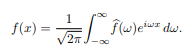
\includegraphics[width=.3\textwidth]{Fourier.png}
	\label{fig:Fourier}
	\caption{Transformada de Fourier para sinais contínuos}
	%\source{Própria}
\end{figure}

\begin{figure}[h]
	\centering
	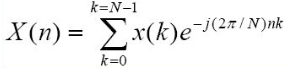
\includegraphics[width=.5\textwidth]{DFT.png}
	\label{fig:DFT}
	\caption{Transformada Discreta de Fourier}
	%\source{Própria}
\end{figure}

As transformadas de Fourier se aplicam somente a sinais de funções estacionárias, onde o espectro de frequência é fixo e não variam com o tempo.

Os sinais de áudio gerados pela voz humana se encontram dentro do espectro de frequências entre 50 a 3400 Hz, e a sua principal característica é a de que a sua frequência não é constante no tempo, o que dá ao sinal da voz humana a característica da não-ergodicidade (seu sinal não mantém as propriedades estatísticas ao longo do tempo), sendo assim, a utilização da STFT (Short Time Fourier Transform) se torna bastante eficaz em sinais dessa natureza.

A STFT é um algoritmo desenvolvido com base na transformada discreta de Fourier, diferenciando-se pela inclusão de uma função de janelamento w(t). Sua principal aplicação é para funções cujo o espectro de frequência varia com o tempo.

\begin{figure}[h]
	\centering
	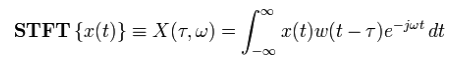
\includegraphics[width=.6\textwidth]{STFT.png}
	\label{fig:STFT}
	\caption{Transformada de Fourier de Tempo Curto}
	%\source{Própria}
\end{figure}

\begin{figure}[h]
	\centering
	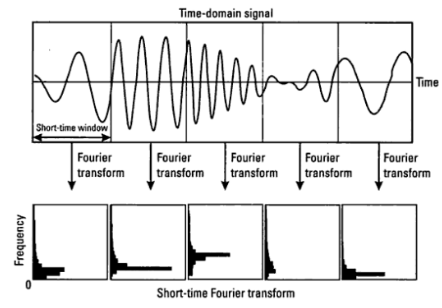
\includegraphics[width=.7\textwidth]{STFT_GRAPHICS.png}
	\label{fig:STFT_GRAPHICS}
	\caption{Transformada de Fourier de Tempo Curto sendo aplicada em diversas frequências de um mesmo sinal}
	%\source{Própria}
\end{figure}
\newpage
 
O principal propósito da utilização de uma STFT é separar o sinal em pequenos intervalos que possam ser tratados individualmente, obtidos através da janela que está inserida na transformada. Desta maneira a modificação de frequência se dá de forma independente, sem a alteração de tempo e vice versa. 

\section*{Funções de Janelamento}
Para aplicações que consistem na amostragem de sinais, a amostragem, por ser finita, resulta em uma forma de onda truncada com características diferentes do sinal original, consequentemente a influência do vazamento espectral torna-se maior para uma situação como esta, gerando uma perda de informação do sinal original. 
Para reduzir os efeitos das imperfeições de amostragem, melhorando a qualidade da reconstrução do sinal é a aplicação de uma função de janelamento.

\begin{figure}[h]
	\centering
	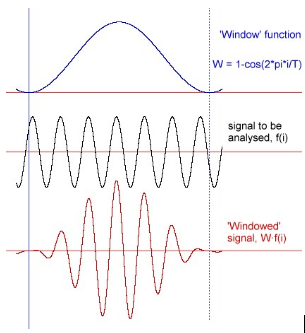
\includegraphics[width=.7\textwidth]{Janelamento.png}
	\label{fig:Janelamento}
	\caption{Efeitos da função de janelamento em um sinal no espectro de frequência}
	%\source{Própria}
\end{figure}
 \newpage

A utilização de uma função de janelamento permite uma definição do período de observação do sinal, redução dos efeitos do vazamento espectral e a separação do sinal de pequena amplitude com frequências muito próximas. A aplicação de uma função de janelamento no tempo, consiste na multiplicação da função original pela função, o que equivale a uma convolução no domínio da frequência.
Existem diversas funções de janelamento, as quais possuem diferentes características e aplicações dependendo principalmente dos parâmetros desejados do sinal original.

\begin{itemize}
	\item Retangular
	\item Hanning
	\item Hamming
	\item Blackman
	\item Kaiser-Bessel
\end{itemize}
 
\section*{Janela Hanning}

Dentre as funções de janelamento existentes, a função Hanning é a mais comumente utilizada na produção musical. O formato desta janela é similar ao de meio ciclo de uma onda cossenoidal. Suas características de baixo vazamento espectral e  formato de onda bem similar ao formato cossenóide,. Torna-se recomendável utilizar portanto a janela para análises de sinais com transientes maiores que de duração da própria janela.

\begin{equation}
w[n] = 0.5-0.5*\cos(\dfrac{2\pi*n}{N}), n = 0, 1, 2,..., N-1 
\end{equation}

\begin{figure}[h]
	\centering
	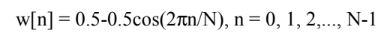
\includegraphics[width=.7\textwidth]{Janela_Hanning.png}
	\label{fig:Janela Hanning}
	\caption{Função da janela Hanning}
	%\source{Própria}
\end{figure}

\begin{figure}[h]
	\centering
	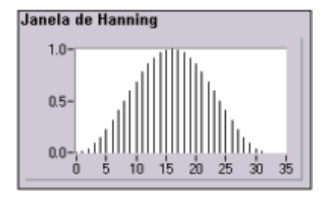
\includegraphics[width=.5\textwidth]{Grafico_Hanning.png}
	\label{fig:Gráfico Hanning}
	\caption{Função da janela Hanning}
	%\source{Própria}
\end{figure}






\chapter{Resultados}
\section{Dados de entrada}
\subsection{Dados Gerais}
A altura escolhida para as torres foi de 0 e 9 para manter a linha de visada direta em paralelo com o chao e assim facilitando os cálculos e diminuindo os erros, os outros dados estão mostrados na tabela abaixo.
	\begin{table}[h]
		\centering
		\begin{tabular}{|
				>{\columncolor[HTML]{DAE8FC}}c |l|}
			\hline
			Distância Total (m) & 0,96713                  \\ \hline
			$\lambda$           & 0,001086957 x  $10^{-6}$ \\ \hline
			Altura das torres   & 0/9                      \\ \hline
		\end{tabular}
	\end{table}
\subsection{Dados dos Obstáculos}

\begin{table}[h]
	\centering
	\begin{tabular}{|
			>{\columncolor[HTML]{DAE8FC}}c |l|}
		\hline
		X                                                   & 325     \\ \hline
		Y                                                   & 7       \\ \hline
		$d_1$                                               & 0,475   \\ \hline
		\multicolumn{1}{|l|}{\cellcolor[HTML]{DAE8FC}$d_2$} & 0,49213 \\ \hline
	\end{tabular}
\end{table}
			
\section{Memorial de Cálculo}
\subsection{Frequência}
Não foi necessário calcular a frequência, o valor utilizado foi de 920MHz e sua escolha está justificada em \ref{sec:esc_freq}.

\subsection{Raio da Parábola}
Com os valores de $X$ e $Y$ do obstáculo o valor encontrado para o raio da parábola foi de:
\begin{equation}
	r_{parabola}= 1,886160714
\end{equation}

\subsection{Atenuação do obstáculo}
Com os valores de $d_1$ e $d_2$ o $\alpha$ encontrado teve valor de :
\begin{equation}
	\alpha = 0,6703932617
\end{equation}

O parâmetro $H_c$ foi encontrado por meio dos dados fornecidos, como mostrado na figura a seguir:

O parâmetro $r_f$ foi cálculado por meio da equação de $Fresnel$, com o valor dos parâmetros a seguir, foi encontrado no gráfico o valor da atenuação do obstáculo.

\begin{table}[h]
	\centering
	\begin{tabular}{|
			>{\columncolor[HTML]{DAE8FC}}c |l|}
		\hline
		$r_f$                                                         & 8,866    \\ \hline
		$H_c$                                                         & 5        \\ \hline
		$\dfrac{H_c}{r_f}$                                            & 0,563    \\ \hline
		\multicolumn{1}{|l|}{\cellcolor[HTML]{DAE8FC}$L_{obstaculo}$} & $22,5dB$ \\ \hline
	\end{tabular}
\end{table}

\subsection{Atenuação no Espaço livre}
Com os valores de $d_1$, $d_2$ e $f$ conhecidos o valor encontrado para $L$ foi:
\begin{equation}
L = 91,43dB
\end{equation}

\subsection{Atenuação total}
A atenuação total consiste nas soma das atenuação encontradas, logo:
\begin{equation}
L_{tot} = L + L_{obstaculo} = 91,43 + 22,5 = 113,9dB 
\end{equation} 

\section{Escolha do tranmissor e da antena}
 A escolha dos módulos e da antena se deu baseado na frequência escolhida para os cálculos e na versatilidade de cada dispositivo. 
 
 O modelo das antenas foi o \textit{Yagi(AirMax Antenna 900Mhz)},devido a sua faixa de trabalho e alta potência.
 
 O modelo do transmissor foi o \textit{Ubiquiti Networks(Rocket M9)} pot ser recomendado para trabalhar em conjunto com o modelo de antena \textit{Yagi}.

\section{Receptor}
Escolha do receptor é encontrado à partir das potências das antenas, do módulo tranmissor e das perdas durante a transmissão. Sua potência foi calculada da seguinte forma:
\begin{equation}
	P_{receptor} = P_{antena_tx} + P_{antena_rx} + P_{transmissor} - L_{tot}
\end{equation}

A mesma antena utilizada para transmissão é utilizada para recepção, os dados da sua potência estão disponíveis nos seu \textit{datasheet} onde $P_{antena_{tx}} = P_{antena_{rx}} = 19dBi$. A potência do transmissõr também está disponível no datasheet, onde $P_{transmissor} = 28dBm$. O valor encontrado para potência do receptor foi de $	P_{receptor} = -47.9dBi$

Com o valor de $-47.9dBi$, o módulo \textit{Ubiquiti Networks(Rocket M9)} também poderá ser utilizado para recepção, tornando o sistema mais simplificado já que ambos receptores e transmissores estarão utilizando antenas recomendadas no datasheet.

\newpage
\begin{center}
	\Large \textbf{Variáveis do projeto}
\end{center}
Todos os valores utilizados e calculados estão registrados na figura a seguir:
\begin{figure}[h]
	\centering
	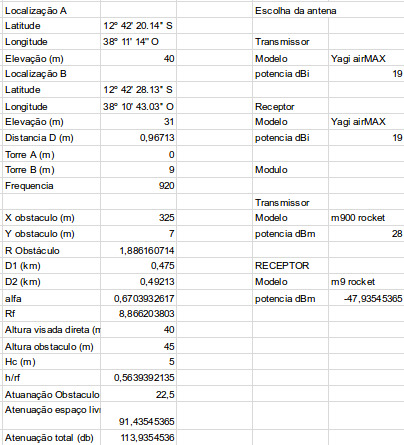
\includegraphics[width=1\textwidth]{resultados.jpeg}
	\label{fig:result}
	\caption{Variáveis do projeto}
	%\source{Própria}
\end{figure} 



%\chapter{Conclusão e Trabalhos Futuros}\label{cap:conclusao}

\lipsum[82-84]

\section{Trabalhos Futuros}

\lipsum[85] 

% ----------------------------------------------------------
% ELEMENTOS PÓS-TEXTUAIS (Referências, Glossário, Apêndices)
% ----------------------------------------------------------
\postextual

\begin{center}
	\Large \textbf{Referências}
\end{center}
	
[1] DANTAS, Joseclécio Dutra, CRUZ, Sérgio da Silva ,Um olhar físico sobre a teoria musical, Universidade Federal de Campina Grande,2018

[2] BERNSSE, Stephan M., Time Stretching And Pitch Shifting of Audio Signals, 2005
	
[3] Gerhard, David Pitch Extraction and Fundamental Frequency: History and Current Techniques, 2003
	
[4] DIAZ, Joe, The fate of Auto-Tune, 2009

[5] Andrade, A. O. e Soares, A. B., Técnicas de Janelamento de Sinais, Universidade Federal de Uberlândia
	
	
	

% Referências bibliográficas
%\bibliography{bibliografia}

%\printglossaries

\thispagestyle{empty}
\vspace*{\fill}
\begingroup
\centering

\huge{ANEXO}

\endgroup
\vspace*{\fill}

\newpage
\textbf{Função GravaAudio}
\\
\lstinputlisting{matlab/gravaAudio.m}

\textbf{Função istft}
\\
\lstinputlisting{matlab/istft.m}

\textbf{Função mostraEspectrograma}
\\
\lstinputlisting{matlab/mostraEspectrograma.m}

\textbf{Função tabelaDoMaior}
\\
\lstinputlisting{matlab/tabelaDoMaior.m}

\textbf{Função compareToPitches}
\\
\lstinputlisting{matlab/compareToPitches.m}

\textbf{Função pitchCorrector}
\\
\lstinputlisting{matlab/compareToPitches.m}

% Índice remissivo (Consultar manual)
%\phantompart
%\printindex



\end{document}
